\documentclass[xcolor=table]{beamer}
\usepackage[table,xcdraw]{xcolor}
\usepackage[utf8]{inputenc}
\usepackage[utf8]{inputenc}
\usepackage{epigraph}
\usepackage{graphicx}
\usepackage[left=25mm,right=25mm,top=2cm,bottom=2cm]{geometry}
\usepackage{indentfirst}
\usepackage{hyperref}
\usepackage{amsmath}
\usepackage{xcolor}
\usepackage{float}
\usepackage{wrapfig}
\usepackage{subfig}
\usepackage[table,xcdraw]{xcolor}
\usepackage[english, russian]{babel}



\usetheme{Madrid}
\usecolortheme{default}

%------------------------------------------------------------
%This block of code defines the information to appear in the
%Title page
\title[Осциллограф] %optional
{Изучение Осциллографа}

%\subtitle{Начало}

\author[Аношин М, Б04-203] % (optional)
{М.~Аношин\inst{1} \and Д.~Лежнев\inst{2}}

%\institute[VFU] % (optional) %adds information about university
%{
%  \inst{1}%
%  Faculty of Physics\\
%  Very Famous University
%  \and
%  \inst{2}%
%  Faculty of Chemistry\\
%  Very Famous University
%}

\date[14.09.2022] % (optional)
{МФТИ, Сентябрь 2022}

%\logo{\includegraphics[height=1cm]{overleaf-logo}}  %adds logo

%End of title page configuration block
%------------------------------------------------------------



%------------------------------------------------------------
%The next block of commands puts the table of contents at the 
%beginning of each section and highlights the current section:

%\AtBeginSection[]
%{
%  \begin{frame}
%    \frametitle{Table of Contents}
%    \tableofcontents[currentsection]
%  \end{frame}
%}
%------------------------------------------------------------


\begin{document}

%The next statement creates the title page.
\frame{\titlepage}


%---------------------------------------------------------
%This block of code is for the table of contents after
%the title page
\begin{frame}
\frametitle{Выбор части}
\tableofcontents
\end{frame}
%---------------------------------------------------------


%---------------------------------------------------------
%Example of the \pause command
%\begin{frame}
%In this slide \pause
%
%the text will be partially visible \pause
%
%And finally everything will be there
%\end{frame}
%---------------------------------------------------------

%---------------------------------------------------------
%Creation of section
\section{Основа устройства осциллографа}

\begin{frame}
\frametitle{Устройство осциллографа}
\begin{figure}
    \centering
    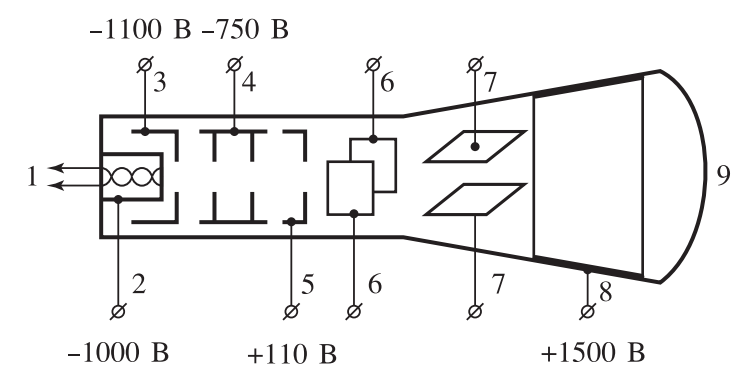
\includegraphics[scale=0.3]{image.png}
    \caption{1 Электронно-лучевая трубка}
    \label{fig:my_label}
\end{figure}
\end{frame}

\begin{frame}
\frametitle{Устройство осциллографа}
\begin{enumerate}
    \item Подогреватель катода
    \item Катод
    \item Модулятор (электрод, управляющий яркостью изображения)
    \item Фокусирующий анод
    \item Ускоряющий анод 
    \item Горизонтально отклоняющие пластины 
    \item Вертикально отклоняющие пластины
    \item Ускоряющий анод
    \item Экран
\end{enumerate}
\end{frame}

\begin{frame}
\frametitle{Устройство осциллографа}
Электрон движется в электрическом поле двух пластин. Пусть его начальная скорость v_0 \text{ вдоль OZ}

Тогда уравнения представляющие движения электрона имеют вид:

\[\dot{ z } = v_0 \Rightarrow z = v_o\cdot t\]
\[m\ddot{ y } = e\cdot{E_y} \Rightarrow  \dot{ y } =  \int \frac{e\cdot{E_y}}{m}\,dt\ = \frac{e\cdot{E_y}\cdot t}{m} \Rightarrow  y = \frac{e\cdot{E_y}\cdot t^2}{2m}\]

Откуда следует, что: \[y = \frac{e\cdot{E_y}}{2m\cdot v_0^2} z^2\]

Видно, что траектория электрона между отклоняющими пластинами
представляет собой параболу. (После выхода из пластин электроны будут двигаться по прямой). Найдём смещение пучка y_1 \text{ и угол }\alpha \text{ между этой прямой и осью z}
\end{frame}

\begin{frame}
\frametitle{Устройство осциллографа}
Пусть к моменту выхода из ускоряющих пластин электрон прошел l вдоль OZ:
\[y_1 = \frac{e\cdot{E_y}}{2m\cdot v_0^2} l^2 \Rightarrow \tan(\alpha) = \frac{y_1}{l} = \frac{e\cdot{E_y}}{2m\cdot v_0^2} l\]
\begin{block}{Внимание!}
Абсолютно такие же действия нужно провести для расчета отклонения вдоль OX
\end{block}
\end{frame}
%---------------------------------------------------------
\section{Усиление, развертка и синхронизация}
\begin{frame}
\frametitle{Усиление сигнала}
Итак, в рабочем режиме координаты x и y точки попадания электронного луча на экран (относительно его центра)
пропорциональны значениям напряжений \math{ U_x(t)}\text{ и }\math{U_y(t)}\text{, где }\math{E_i = \frac{U_i}{d}, } \text{ а d - растояние между пластинами}

\large \large Ясно, что отклонение луча должно быть не должно выходить за пределы экрана. Что подводит нас к мысле о необходимости усиления(ослабления) сигнала

Для усиления слабых сигналов в осциллографе имеются усилители вертикального (и горизонтального) отклонения
луча. \[K_y = U_y/h_y, K_x = U_x/h_x - \]  \text{отношение величины поданного напряжения к смещению луча }

на экране.
\end{frame}

\begin{frame}
\frametitle{Развёртка сигнала}
Для развертки сигнала, нужно подавать такое напряжение U_i:
U_i(t) = U_{0i} + K_i \cdot U(t), \text{что будет изменятся со временем, вынуждая картирнку}

на экране доходить до конца и обратно
\begin{figure}
    \centering
    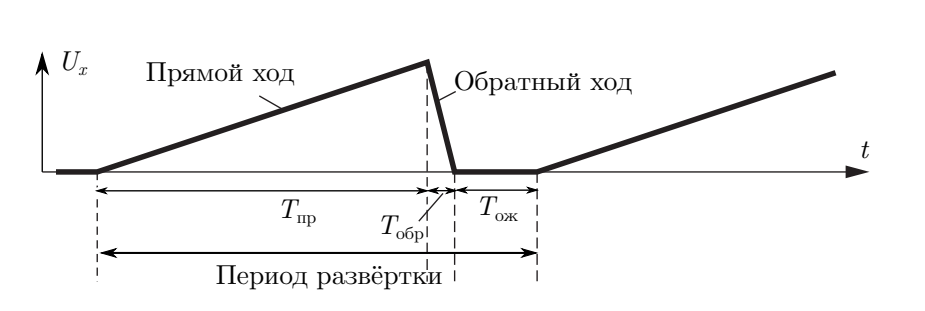
\includegraphics[scale=0.3]{Screenshot from 2022-09-14 20-14-31.png}
    \caption{2 Напряжение развёртки}
    \label{fig:my_label}
\end{figure}
(Tобр \ll Tпр)
\end{frame}

\begin{frame}
\frametitle{Синхронизация}
Для получения статичной картины на экране осциллографа необходимо, чтобы
период развёртки был кратен периоду изучаемого периодического сигнала — тогда повторная «прорисовка» пройдёт по тому же пути, что и предыдущая. Но полная сихронизация трудно выполнима из-за неточностей и генератора, и осциллографа. В таком случае применяют
\textbf{принудительное согласование периодов}, при котором напряжение U(t) «навязывает» свой
период генератору развёртки. При этом начало прямого
хода развёртки должно совпадать строго с одной и той же характерной точкой исследуемого периодического сигнала
    
\end{frame}
%---------------------------------------------------------
%Highlighting text
%\begin{frame}
%\frametitle{Sample frame title}
%
%In this slide, some important text will be
%\alert{highlighted} because it's important.
%Please, don't abuse it.
%
%\begin{block}{Remark}
%Sample text
%\end{block}
%
%\begin{alertblock}{Important theorem}
%Sample text in red box
%\end{alertblock}
%
%\begin{examples}
%Sample text in green box. The title of the block is ``Examples".
%\end{examples}
%\end{frame}
%---------------------------------------------------------
\section{Ход лабораторной работы работа}
\begin{frame}
\frametitle{Последовательность дейстивий}
\begin{enumerate}
    \item Включаение осциллографа. Подгтовка к работе, прогрев прибора
    \item Проведение первой серии измерений для синусоиды, полученной осциллографом от велечины исходного сигнала генератора
    \item Проведение второй серии измерений для амплитулы, работа с понижением сигнала на -20dB и -40dB 
    \item Проведение третиий серии измерений для фигур Лиссажу, полученных на экране осциллографа 
    \item Проведение четвертой серии измерений для определения коэффициента ослабления АЧХ осциллографа
    \item Анализ полученных зависмостей и заключение о результатах экспериментов
\end{enumerate}
\end{frame}

\begin{frame}
\frametitle{Результаты первой серии измерений}    
\resizebox{11cm}{!}{
    \begin{table}[]
    \begin{tabular}{rrlrrrr}
    \rowcolor[HTML]{FBBC04} 
    \multicolumn{1}{l}{\cellcolor[HTML]{FBBC04}\textit{\textbf{\nu_{ЗГ}\text{, Гц}}}} &
      \multicolumn{1}{l}{\cellcolor[HTML]{FBBC04}\textit{\textbf{T, дел}}} &
      \textit{\textbf{TIME/DIV}} &
      \multicolumn{1}{l}{\cellcolor[HTML]{FBBC04}\textit{\textbf{T, с}}} &
      \multicolumn{1}{l}{\cellcolor[HTML]{FBBC04}\textit{\textbf{\nu\text{, Гц}}}} &
      \multicolumn{1}{l}{\cellcolor[HTML]{FBBC04}\textit{\textbf{\delta\nu\text{, Гц}}}} &
      \multicolumn{1}{l}{\cellcolor[HTML]{FBBC04}\textit{\textbf{\nu − ν_{ЗГ}\text{, Гц}}}} \\
    \cellcolor[HTML]{FFFFFF}\textit{997.6} & 10 & 0.5 ms                          & 0.001   & 1000    & 50     & 2.4    \\
    \cellcolor[HTML]{FFFFFF}\textit{58.8}  & 17 & \cellcolor[HTML]{FFFFFF}5    ms & 0.017   & 58.82   & 1.73   & 0.02   \\
    298.4                                           & 17 & 2    ms                         & 0.0034  & 294.12  & 8.7    & -4.28  \\
    603.2                                           & 17 & 1    ms                         & 0.0017  & 588.24  & 17.3   & -14.96 \\
    1999.3                                          & 13 & 0.2 ms                          & 0.00052 & 1923.08 & 73.96  & -76.22 \\
    5000.3                                          & 10 & 0.1 ms                          & 0.0002  & 5000.00 & 250.00 & -0.30 
    \end{tabular}
    \end{table}
}

\textbf{Для 2 - 5 написаны деления для двух периодов, для повышения точности}				
\end{frame}

\begin{frame}
\frametitle{Результаты второй серии измерений}    
\resizebox{11cm}{!}{
    \begin{table}[]
    \begin{tabular}{llllll}
     &
      \cellcolor[HTML]{FBBC04}\textit{\textbf{U, В}} &
      \cellcolor[HTML]{FBBC04}\textit{\textbf{VOLTS/DIV}} &
      \cellcolor[HTML]{FBBC04}\textit{\textbf{T, дел}} &
      \cellcolor[HTML]{FBBC04}\textit{\textbf{dU\_max, В}} &
      \cellcolor[HTML]{FBBC04}\textit{\textbf{dU\_max/U\_max}} \\
    \cellcolor[HTML]{FBBC04}\textit{\textbf{U\_max, В}} &
      \multicolumn{1}{r}{7.2} &
      \multicolumn{1}{r}{2} &
      \multicolumn{1}{r}{36} &
      \multicolumn{1}{r}{0.2} &
      \multicolumn{1}{r}{0.028} \\
    \cellcolor[HTML]{FBBC04}\textit{\textbf{U\_min, В}} &
      \multicolumn{1}{r}{0.56} &
      \multicolumn{1}{r}{0.2} &
       &
      \multicolumn{1}{r}{0.02} &
      \multicolumn{1}{r}{0.036} \\
     &
       &
       &
       &
       &
      
    \end{tabular}
    \end{table}
}

\textbf{Для 2 - 5 написаны деления для двух периодов, для повышения точности}				
\end{frame}

\begin{frame}
\frametitle{Результаты второй серии измерений}    
\resizebox{11cm}{!}{
    \begin{table}[]
    \begin{tabular}{rrlrrrr}
    \rowcolor[HTML]{FBBC04} 
    \multicolumn{1}{l}{\cellcolor[HTML]{FBBC04}\textit{\textbf{}}} &
      \multicolumn{1}{l}{\cellcolor[HTML]{FBBC04}\textit{\textbf{U\_max, В}}} &
      \textit{\textbf{VOLTS/DIV}} &
      \multicolumn{1}{l}{\cellcolor[HTML]{FBBC04}\textit{\textbf{T, дел}}} &
      \multicolumn{1}{l}{\cellcolor[HTML]{FBBC04}\textit{\textbf{}}} &
      \multicolumn{1}{l}{\cellcolor[HTML]{FBBC04}\textit{\textbf{}}} &
      \multicolumn{1}{l}{\cellcolor[HTML]{FBBC04}\textit{\textbf{}}} \\
    \multicolumn{1}{l}{\cellcolor[HTML]{FBBC04}\textit{\textbf{-40dB}}} & 0.12 & \multicolumn{1}{r}{0.2}                         & 6  &  &  &  \\
    \multicolumn{1}{l}{\cellcolor[HTML]{FBBC04}\textit{\textbf{-20dB}}} & 1.1  & \multicolumn{1}{r}{\cellcolor[HTML]{FFFFFF}0.5} & 22 &  &  &  \\
                                                                        &      &                                                 &    &  &  &  \\
                                                                        &      &                                                 &    &  &  &  \\
                                                                        &      &                                                 &    &  &  &  \\
                                                                        &      &                                                 &    &  &  & 
    \end{tabular}
    \end{table}
}
\textbf{Деления для двух периодов, для повышения точности}				
\end{frame}

\begin{frame}
\frametitle{Результаты третьей серии измерений}
\begin{figure}%
    \centering
    \subfloat[\centering {\nu_1}:{\nu_2} = 2:3]{{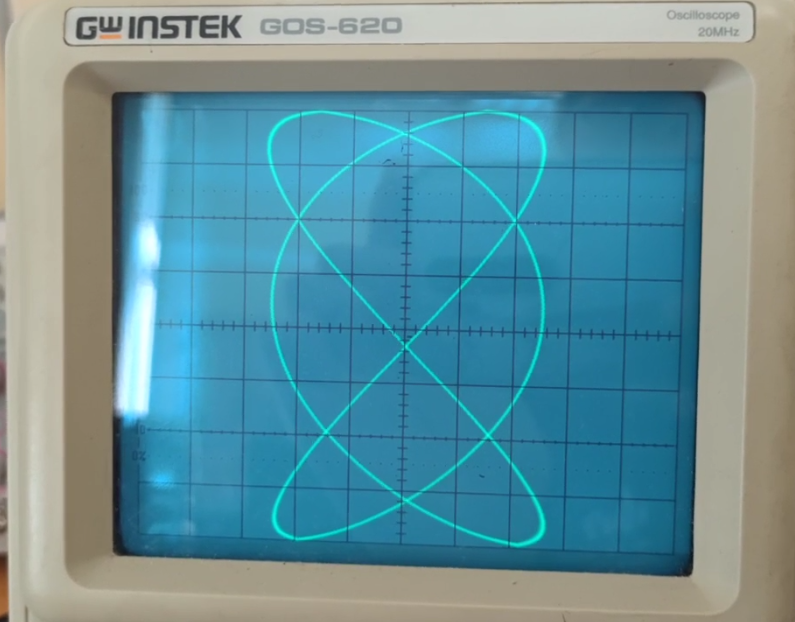
\includegraphics[width=5cm]{Screenshot from 2022-09-14 21-07-32.png} }}%
    \qquad
    \subfloat[\centering {\nu_1}:{\nu_2} = 1:3]{{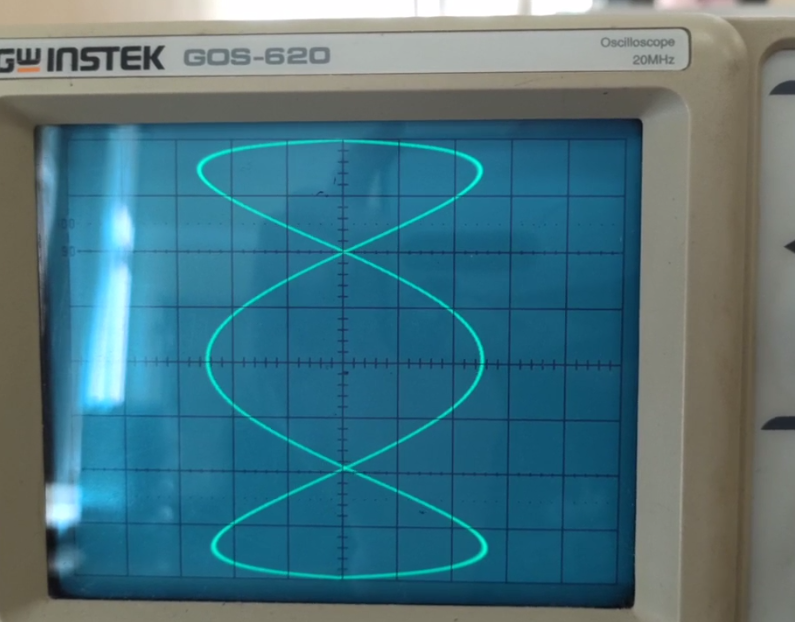
\includegraphics[width=5cm]{Screenshot from 2022-09-14 21-09-38.png} }}%
    \caption{3 Фигуры Лиссажу, часть 1}%
    \label{fig:example}%
\end{figure}
\end{frame}

\begin{frame}
\frametitle{Результаты третьей серии измерений}
\begin{figure}
    \centering
    \subfloat[\centering {\nu_1}:{\nu_2} = 1:2]{{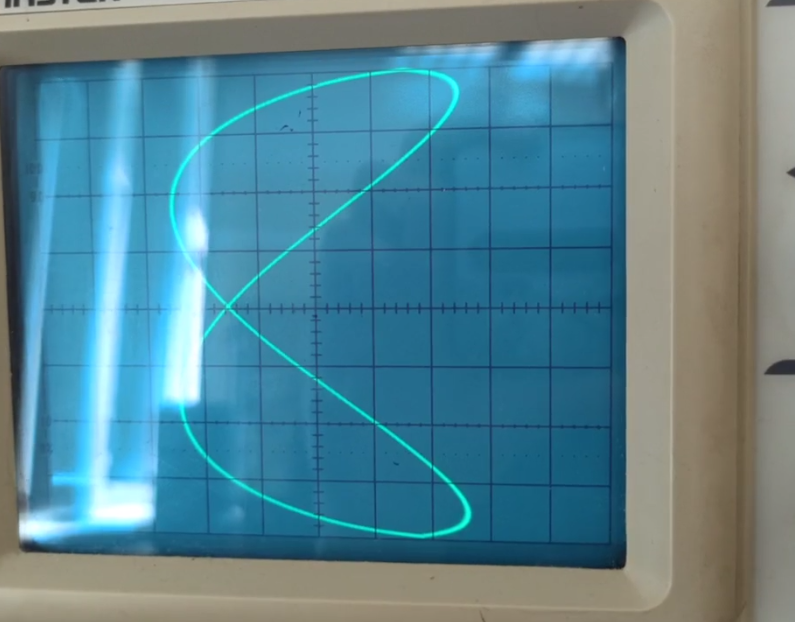
\includegraphics[width=5cm]{Screenshot from 2022-09-14 21-13-26.png} }}%
    \qquad
    \subfloat[\centering {\nu_1}:{\nu_2} = 1:1]{{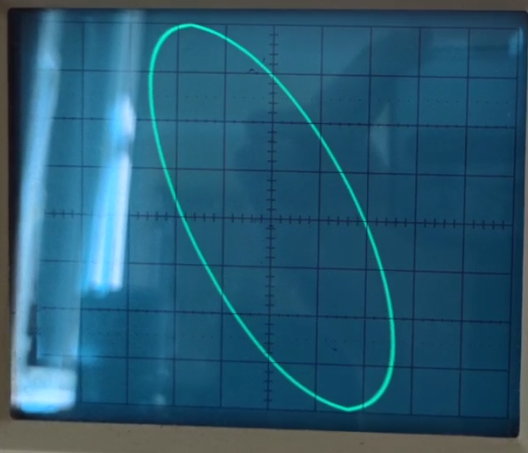
\includegraphics[width=5cm]{Screenshot from 2022-09-14 21-15-17.png} }}%
    \caption{4 Фигуры Лиссажу, часть 2}%
    \label{fig:example}%
\end{figure}
\end{frame}

\begin{frame}
\frametitle{Результаты третьей серии измерений}
\begin{figure}
    \centering
    \subfloat[\centering {\nu_1}:{\nu_2} = 2:5]{{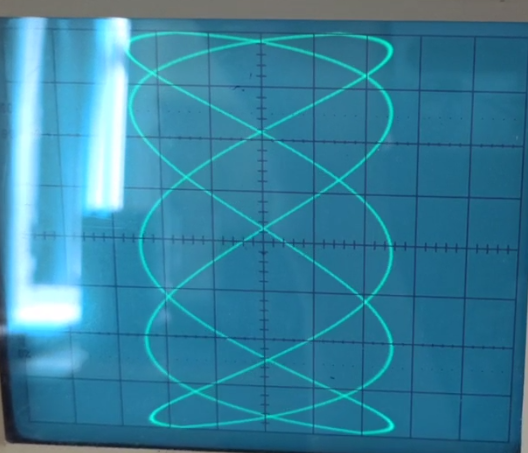
\includegraphics[width=5cm]{Screenshot from 2022-09-14 21-17-29.png} }}%
    \qquad
    \subfloat[\centering {\nu_1}:{\nu_2} = 2:3]{{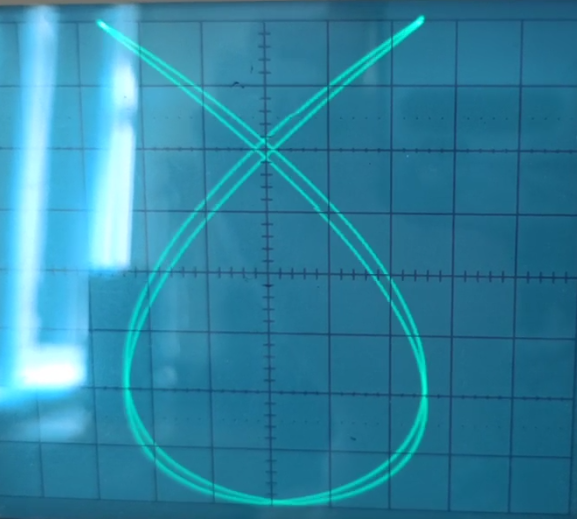
\includegraphics[width=5cm]{Screenshot from 2022-09-14 21-19-22.png} }}%
    \caption{5 Фигуры Лиссажу, часть 3}%
    \label{fig:example}%
\end{figure}
\end{frame}

\begin{frame}
\frametitle{Результаты четвертой серии измерений}
\resizebox{11cm}{!}{
    \begin{table}[]
    \begin{tabular}{rrlrrrr}
    \rowcolor[HTML]{FBBC04} 
    \multicolumn{1}{l}{\cellcolor[HTML]{FBBC04}\textit{\textbf{}}} &
      \multicolumn{1}{l}{\cellcolor[HTML]{FBBC04}\textit{\textbf{Umax/U−20dB}}} &
      \textit{\textbf{U−20dB/U−40dB}} &
      \multicolumn{1}{l}{\cellcolor[HTML]{FBBC04}\textit{\textbf{U−40dB/Umin}}} &
      \multicolumn{1}{l}{\cellcolor[HTML]{FBBC04}\textit{\textbf{}}} &
      \multicolumn{1}{l}{\cellcolor[HTML]{FBBC04}\textit{\textbf{}}} &
      \multicolumn{1}{l}{\cellcolor[HTML]{FBBC04}\textit{\textbf{}}} \\
    \multicolumn{1}{l}{\cellcolor[HTML]{FBBC04}\textit{\textbf{-40dB}}} & 16.319 & \multicolumn{1}{r}{19.24}                       & -13.380 &  &  &  \\
    \multicolumn{1}{l}{\cellcolor[HTML]{FBBC04}\textit{\textbf{-20dB}}} & 1.1    & \multicolumn{1}{r}{\cellcolor[HTML]{FFFFFF}0.5} & 22      &  &  &  \\
                                                                        &        &                                                 &         &  &  &  \\
                                                                        &        &                                                 &         &  &  &  \\
                                                                        &        &                                                 &         &  &  &  \\
                                                                        &        &                                                 &         &  &  & 
    \end{tabular}
    \end{table}
}
\resizebox{6cm}{!}{
    \begin{table}[]
    \begin{tabular}{rrlrrrr}
    \rowcolor[HTML]{FBBC04} 
    \multicolumn{1}{l}{\cellcolor[HTML]{FBBC04}\textit{\text{\nu\text{, Гц}}}} &
      \multicolumn{1}{l}{\cellcolor[HTML]{FBBC04}\textit{\text{U, В}}}\\
    1000    & 4   & \multicolumn{1}{r}{}                         &  &  &  &  \\
    30000000 & 3.4 & \multicolumn{1}{r}{\cellcolor[HTML]{FFFFFF}} &  &  &  &  \\
    23115000                                           & 3.8 &                                              &  &  &  &  \\
    23000000                                           & 3.8 &                                              &  &  &  &  \\
    100                                                & 4   &                                              &  &  &  &  \\
    10                                                 & 4   &                                              &  &  &  & 
    \end{tabular}
    \end{table}
}
\end{frame}

\begin{frame}
\frametitle{Обработка данных:}
\resizebox{6cm}{!}{
    \begin{table}[]
    \begin{tabular}{rr}
    \rowcolor[HTML]{FBBC04} 
    \multicolumn{1}{l}{\cellcolor[HTML]{FBBC04}\textit{\text{K(\nu) = U(\nu):U_0}}} & \multicolumn{1}{l}{\cellcolor[HTML]{FBBC04}\textit{\text{U, В}}} \\
    0.85 & 3.4 \\
    0.95 & 3.8 \\
    0.95 & 3.8 \\
    1    & 4   \\
    100  & 4   \\
    10   & 4  
    \end{tabular}
    \end{table}
}

Полученные коэффициенты ослабления АЧХ говорят о том, что осциллограф способен качественно обрабатывать сигнал на всей полосе пропускания, т.к увелечение частоты в 30 тысяч раз увеличило помехи лишь в 1.17 раза
\end{frame}
%---------------------------------------------------------
%Two columns
%\begin{frame}
%\frametitle{Two-column slide}

%\begin{columns}
%
%\column{0.5\textwidth}
%This is a text in first column.
%$$E=mc^2$$
%\begin{itemize}
%\item First item
%\item Second item
%\end{itemize}
%
%\column{0.5\textwidth}
%This text will be in the second column
%and on a second tought this is a nice looking
%layout in some cases.
%\end{columns}
%\end{frame}
%---------------------------------------------------------


\end{document}